\documentclass{beamer}

\usepackage{fontspec}
\usepackage{xeCJK}
\setCJKmainfont{DFFN_R3.TTC}
\XeTeXlinebreaklocale "zh"
\XeTeXlinebreakskip = 0pt plus 1pt
\linespread{1.3}
\allowdisplaybreaks

\newcommand{\weib}{\CJKfamily{weib}}
\newcommand{\hkss}{\CJKfamily{hkss}}
\newcommand{\hksy}{\CJKfamily{hksy}}
\newcommand{\lth}{\CJKfamily{lth}}
\usepackage{color}
\usepackage{booktabs}
\usepackage{tabularx}
\usepackage{caption}
\usepackage{tikz}
\usepackage{verbatim}
\usepackage{pgfplotstable}
\pgfplotsset{width=12cm}
\pgfplotsset{height=7cm}
\pgfplotsset{compat=1.13}

\usetheme{EastLansing}
\usetikzlibrary{positioning}
\useinnertheme{rectangles}
\usefonttheme{professionalfonts}

\newcommand{\lw}{0.8mm}
\setbeamercovered{transparent}


%\AtBeginSection[]
%{
  %\begin{frame}<beamer>
	%\frametitle{報告大綱}
	%%\frametitle{RoadMap}
    %\tableofcontents[currentsection]
  %\end{frame}
%}

\title{Paper Introduction}
\subtitle{\textcolor[rgb]{0.00,0.50,1.00}{{Speech Processing \& Machine Learning Laboratory}}}
\author{徐瑞陽}
\date{2019/06/12}
\begin{document}

\begin{frame}
\maketitle
\end{frame}

\begin{frame}
\frametitle{Outline}
\tableofcontents
\end{frame}


\section{Meta Learning}
\begin{frame}
  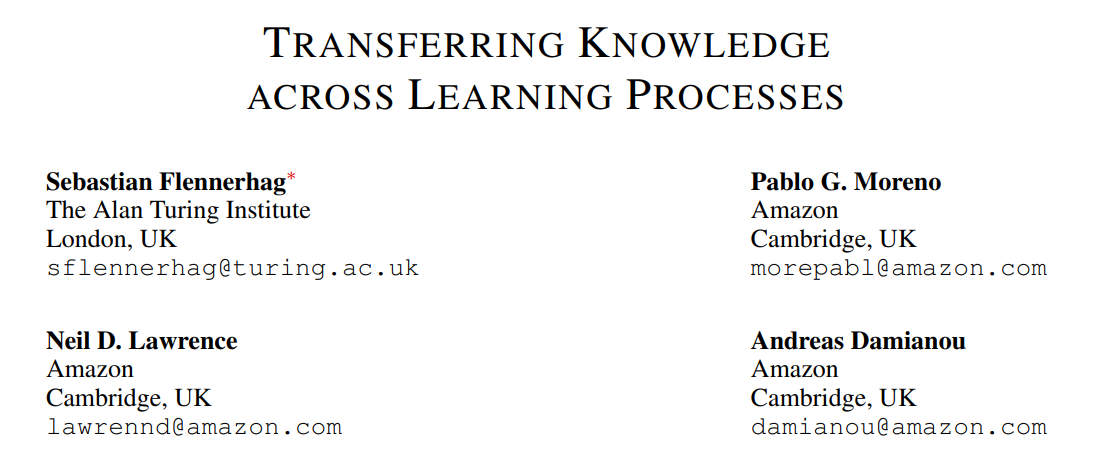
\includegraphics[width=\textwidth]{fig/p1-title.png}
  \center ICLR 2019
  \center (6,8,8)
\end{frame}

\begin{frame}{Motivation}
  Current meta-learning algorithm mainly focus on \textbf{few-shot learning} problem. 
  \begin{itemize}
    \item Few samples for each task
    \item Few gradient steps (to avoid overfitting)
  \end{itemize}
\end{frame}

\begin{frame}{Motivation}
  Can we extend meta-learning to more complex task?
  \begin{itemize}
    \item \textbf{low-resource} rather than \textbf{few-shot}
    \item \textbf{rapid adaptation} (e.g thousands of gradient steps) rather than \textbf{few} gradient steps
  \end{itemize}
\end{frame}

\begin{frame}{Highlight}
  \begin{itemize}
    \item New meta-objective
    \item More realistic experiment settings
  \end{itemize}
\end{frame}

\begin{frame}{New meta-objective}
  \begin{itemize}
    \item The length of learning process is small
    \item The learning process is smooth
  \end{itemize}

\end{frame}

\begin{frame}{New meta-objective}
  Minimize the travelling length in a task manifold $M$

  \begin{itemize}
    \item $p = (\theta,f(\theta)) \in M$
    \item $f(\cdot)$: objective function
  \end{itemize}
  \center 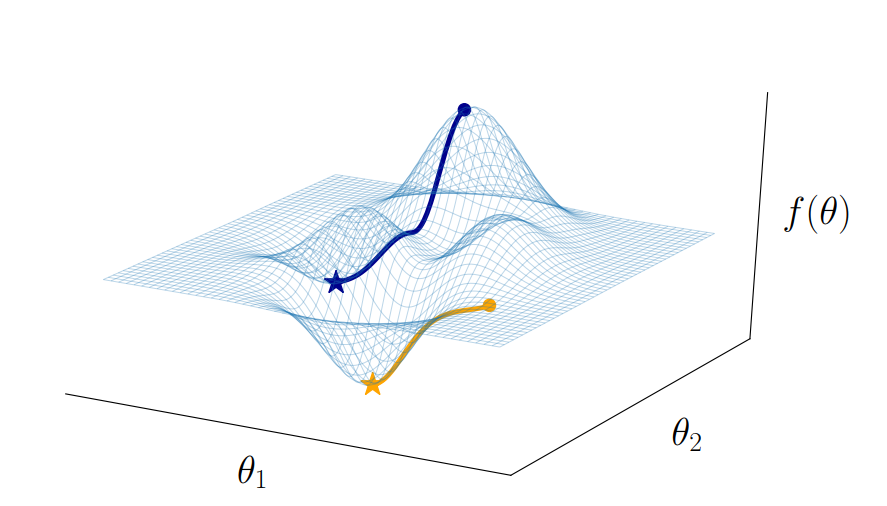
\includegraphics[width=0.7 \textwidth]{fig/p1-manifold.png}
\end{frame}

\begin{frame}{Idea}
\center 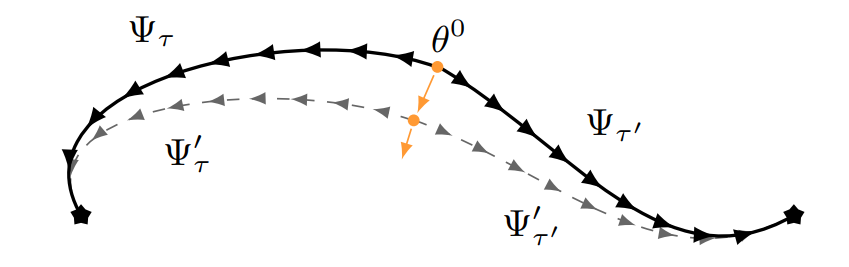
\includegraphics[width = \textwidth]{fig/p1-idea.png}
\end{frame}


\begin{frame}{Some notation about learning process}
  \begin{itemize}
    \item learning process $\gamma$ is a curve on $M$
    \item $\gamma^i$ is the $i$-th point on $\gamma$ (discrete version)
    \item distance metric $d(\theta^0;M) = \sum_{i=0}^{K-1} ||\gamma^{i+1} - \gamma^i||_2$
  \end{itemize}
\end{frame}

\begin{frame}
  \begin{block}{Meta objective}
  \[
    \theta^{\star} = \arg\min_{\theta^0} F(\theta^0) = \mathbb{E}_{\tau \sim p(\tau)} [\, d(\theta^0;M_\tau) ]\,
  \]
  \end{block}

  \begin{itemize}
    \item $\theta_{\tau}^{i+1} = u_\tau(\theta^i_\tau), \quad \theta_\tau^0 = \theta^0 \, \text{is shared across tasks}$
    \item $\theta^0 \in \Theta = \cap_\tau \lbrace \theta^0 | f_\tau(\theta_\tau^{K_\tau}) \leq f_\tau(\psi_\tau^{K_\tau}) \rbrace$
    \item $\psi_\tau^0$ can be random initialization or pretrained weights
  \end{itemize}
\end{frame}

\begin{frame}{時光屋}
  \begin{itemize}
    \item Combine second constraint into distance metric
    \item Approximate Jacobian matrix of $\theta^0$ as Identity matrix
    \item And some approximations...
  \end{itemize}
\end{frame}

\begin{frame}{Meta gradient}
  \[
    \nabla F(\theta^0) = \mathbb{E}_{\tau \sim p(\tau)} \Big [\, \sum_{i=0}^{K_\tau - 1} \Delta f_\tau^i \nabla f_\tau(\theta_\tau^i) + \Delta \theta_\tau^i \Big]\,
  \]

  \begin{itemize}
    \item FOMAML: $\mathbb{E}_{\tau \sim p(\tau)} \Big [\, \nabla f_\tau(\theta^{K_\tau -1}_\tau) \Big ]\,$ 
    \item Reptile: $\mathbb{E}_{\tau \sim p(\tau)} \Big [\, \sum_{i=0}^{K_\tau - 1} \Delta \theta_\tau^i \Big ]\,$
  \end{itemize}
\end{frame}

\section{MISC}
\begin{frame}
	\begin{center}
    %\weib{\LARGE{謝謝聆聽!}}
    \LARGE{Questions?}
	\end{center}
\end{frame}


\subsection{Appendix}
\end{document} 
